% Meta-ORES entities and their relationships.
\documentclass{article}
\usepackage{tikz}
\usepackage[strict]{changepage}
\usetikzlibrary{arrows,shapes}

% Disable page number for better SVG.
\pagenumbering{gobble}

\begin{document}
\begin{adjustwidth}{-8em}{}
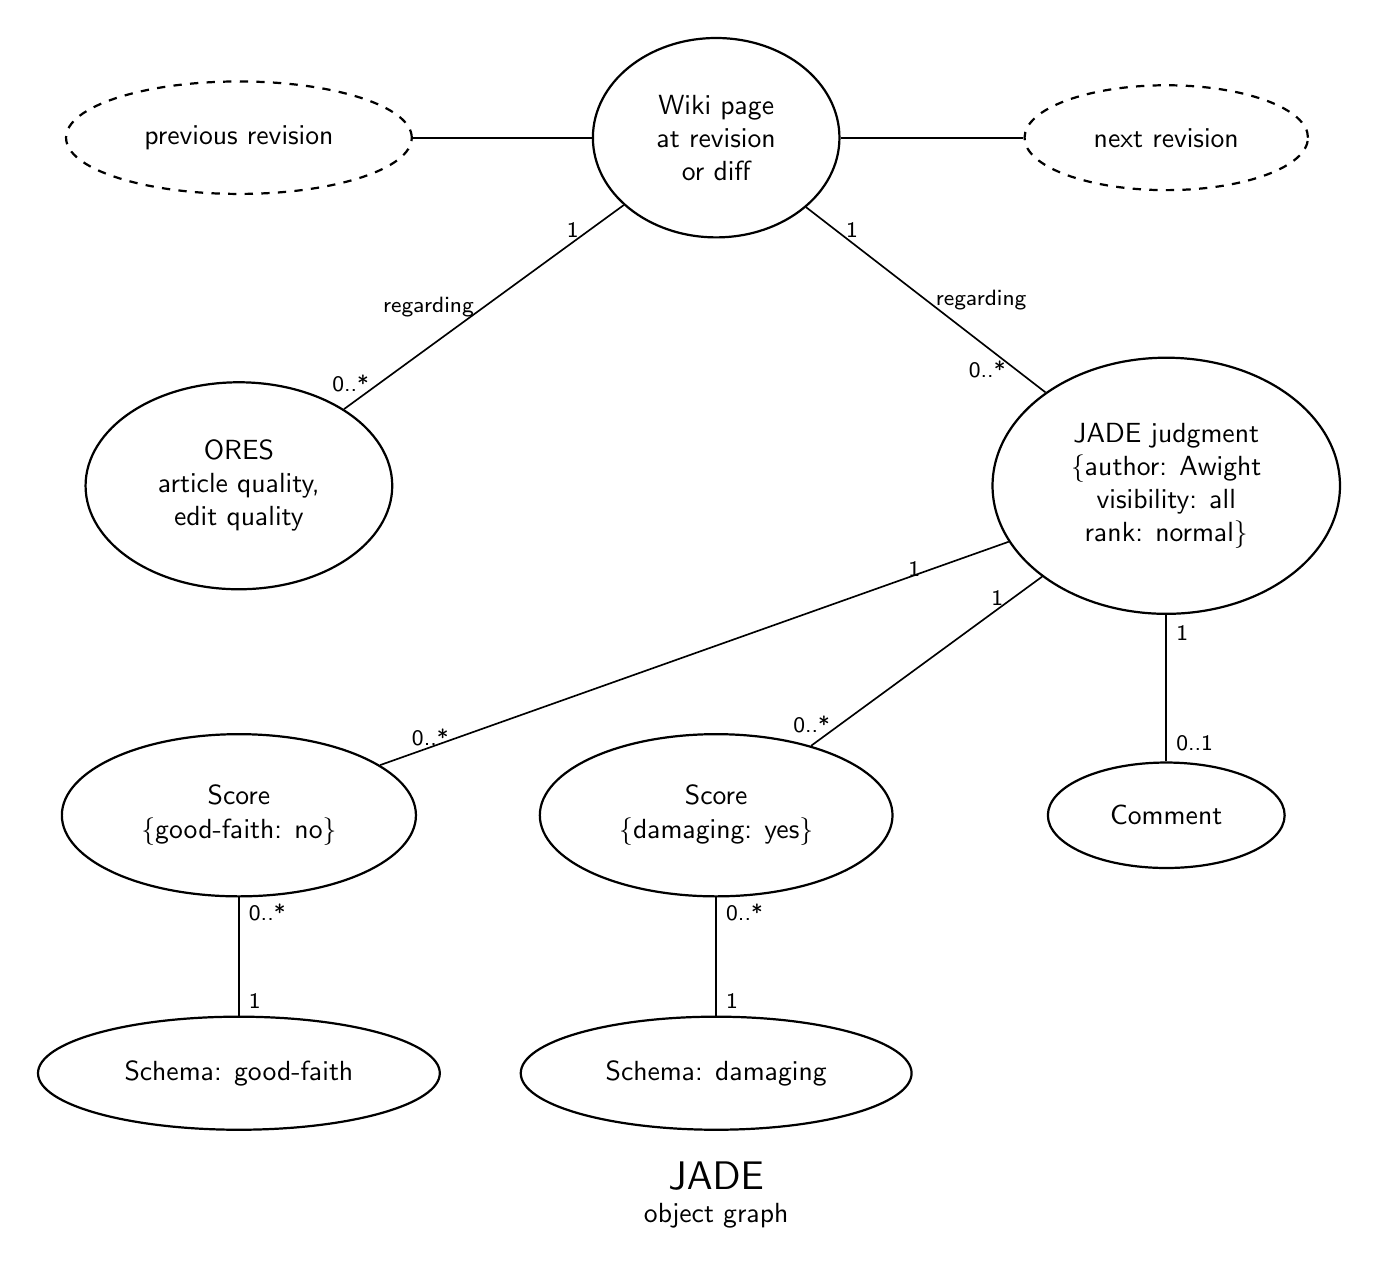
\begin{tikzpicture}[
  font=\sffamily,
  every matrix/.style={ampersand replacement=\&, column sep=1cm, row sep=1.5cm, fill=white},
  entity/.style={draw, ellipse, thick, inner sep=1em},
  other-entity/.style={draw, ellipse, thick, inner sep=1em, dashed},
  arrow/.style={->, >=stealth', shorten >=1pt, semithick, font=\sffamily\footnotesize},
  line/.style={-, semithick, font=\sffamily\footnotesize},
  every node/.style={align=center}]

  % TODO: dashed boxes for regions: wiki entity, judgment, discussion

  % Position the nodes using a matrix layout
  \matrix{
    \node[other-entity] (previous) {previous revision};
      \& \node[entity] (artifact) {Wiki page \\ at revision \\ or diff};
        \& \node[other-entity] (next) {next revision}; \\
    \node[entity] (ores-scores) {ORES \\ article quality, \\ edit quality};
        \& \& \node[entity] (judgment) {JADE judgment \\ \{author: Awight \\ visibility: all \\ rank: normal\}}; \\
    \node[entity] (score1) {Score \\ \{good-faith: no\}};
      \& \node[entity] (score2) {Score \\ \{damaging: yes\}};
        \& \node[entity] (comment) {Comment}; \\
    \node[entity] (schema1) {Schema: good-faith};
      \& \node[entity] (schema2) {Schema: damaging}; \\
  };

  % Draw the lines between the nodes and label them.
  \draw[line] (ores-scores) --
    node[very near start, left] {0..*}
    node[midway, left] {regarding}
    node[very near end, left] {1}
    (artifact);
  \draw[line] (judgment) --
    node[very near start, left] {0..*}
    node[midway, right] {regarding}
    node[very near end, right] {1}
    (artifact);
  \draw[line] (previous) -- (artifact);
  \draw[line] (artifact) -- (next);
  \draw[line] (score1) --
    node[very near start, left] {0..*}
    node[very near end, left] {1}
    (judgment);
  \draw[line] (score2) --
    node[very near start, left] {0..*}
    node[very near end, left] {1}
    (judgment);
  \draw[line] (comment) --
    node[very near start, right] {0..1}
    node[very near end, right] {1}
    (judgment);
  \draw[line] (schema1) --
    node[very near start, right] {1}
    node[very near end, right] {0..*}
    (score1);
  \draw[line] (schema2) --
    node[very near start, right] {1}
    node[very near end, right] {0..*}
    (score2);

  \node [below=1cm, align=flush center] at (schema2)
  {\Large JADE \\ \normalsize object graph};

\end{tikzpicture}
\end{adjustwidth}
\end{document}
